
\documentclass[11pt,a4paper]{report}%especifica o tipo de documento que tenciona escrever: carta, artigo, relatório... neste caso é um relatório
% [11pt,a4paper] Define o tamanho principal das letras do documento. caso não especifique uma delas, é assumido 10pt
% a4paper -- Define o tamanho do papel.

\usepackage[portuges]{babel}%Babel -- irá activar automaticamente as regras apropriadas de hifenização para a língua todo o
                                   %-- o texto gerado é automaticamente traduzido para Português.
                                   %  Por exemplo, “chapter” irá passar a “capítulo”, “table of contents” a “conteúdo”.
                                   % portuges -- específica para o Português.
\usepackage[utf8]{inputenc} % define o encoding usado texto fonte (input)--usual "utf8" ou "latin1

\usepackage{graphicx} %permite incluir graficos, tabelas, figuras
\usepackage{url} % para utilizar o comando \url{}
\usepackage{enumerate} %permite escolher, nas listas enumeradas, se os iems sao marcados com letras ou numeros-romanos em vez de numeracao normal

%\usepackage{apalike} % gerar biliografia no estilo 'named' (apalike)

\usepackage{color} % Para escrever em cores

\usepackage{multirow} %tabelas com multilinhas
\usepackage{array} %formatação especial de tabelas em array

\usepackage[pdftex]{hyperref} % transformar as referências internas do seu documento em hiper-ligações.

%Exemplos de fontes -- nao e vulgar mudar o tipo de fonte
%\usepackage{tgbonum} % Fonte de letra: TEX Gyre Bonum
%\usepackage{lmodern} % Fonte de letra: Latin Modern Sans Serif
%\usepackage{helvet}  % Fonte de letra: Helvetica
%\usepackage{charter} % Fonte de letra:Charter

\definecolor{saddlebrown}{rgb}{0.55, 0.27, 0.07} % para definir uma nova cor, neste caso 'saddlebrown'

\usepackage{listings}  % para utilizar blocos de texto verbatim no estilo 'listings'
%paramerização mais vulgar dos blocos LISTING - GENERAL
\lstset{
	basicstyle=\small, %o tamanho das fontes que são usadas para o código
	numbers=left, % onde colocar a numeração da linha
	numberstyle=\tiny, %o tamanho das fontes que são usadas para a numeração da linha
	numbersep=5pt, %distancia entre a numeração da linha e o codigo
	breaklines=true, %define quebra automática de linha
    frame=tB,  % caixa a volta do codigo
	mathescape=true, %habilita o modo matemático
	escapeinside={(*@}{@*)} % se escrever isto  aceita tudo o que esta dentro das marcas e nao altera
}
%
%\lstset{ %
%	language=Java,							% choose the language of the code
%	basicstyle=\ttfamily\footnotesize,		% the size of the fonts that are used for the code
%	keywordstyle=\bfseries,					% set the keyword style
%	%numbers=left,							% where to put the line-numbers
%	numberstyle=\scriptsize,				% the size of the fonts that are used for the line-numbers
%	stepnumber=2,							% the step between two line-numbers. If it's 1 each line
%											% will be numbered
%	numbersep=5pt,							% how far the line-numbers are from the code
%	backgroundcolor=\color{white},			% choose the background color. You must add \usepackage{color}
%	showspaces=false,						% show spaces adding particular underscores
%	showstringspaces=false,					% underline spaces within strings
%	showtabs=false,							% show tabs within strings adding particular underscores
%	frame=none,								% adds a frame around the code
%	%abovecaptionskip=-.8em,
%	%belowcaptionskip=.7em,
%	tabsize=2,								% sets default tabsize to 2 spaces
%	captionpos=b,							% sets the caption-position to bottom
%	breaklines=true,						% sets automatic line breaking
%	breakatwhitespace=false,				% sets if automatic breaks should only happen at whitespace
%	title=\lstname,							% show the filename of files included with \lstinputlisting;
%											% also try caption instead of title
%	escapeinside={\%*}{*)},					% if you want to add a comment within your code
%	morekeywords={*,...}					% if you want to add more keywords to the set
%}

\usepackage{xspace} % deteta se a seguir a palavra tem uma palavra ou um sinal de pontuaçao se tiver uma palavra da espaço, se for um sinal de pontuaçao nao da espaço

\parindent=0pt %espaço a deixar para fazer a  indentação da primeira linha após um parágrafo
\parskip=2pt % espaço entre o parágrafo e o texto anterior

\setlength{\oddsidemargin}{-1cm} %espaço entre o texto e a margem
\setlength{\textwidth}{18cm} %Comprimento do texto na pagina
\setlength{\headsep}{-1cm} %espaço entre o texto e o cabeçalho
\setlength{\textheight}{23cm} %altura do texto na pagina

% comando '\def' usado para definir abreviatura (macros)
% o primeiro argumento é o nome do novo comando e o segundo entre chavetas é o texto original, ou sequência de controle, para que expande
\def\darius{\textsf{Darius}\xspace}
\def\antlr{\texttt{AnTLR}\xspace}
\def\pe{\emph{Publicação Eletrónica}\xspace}
\def\titulo#1{\section{#1}}    %no corpo do documento usa-se na forma '\titulo{MEU TITULO}'
\def\super#1{{\em Supervisor: #1}\\ }
\def\area#1{{\em \'{A}rea: #1}\\[0.2cm]}
\def\resumo{\underline{Resumo}:\\ }

%\input{LPgeneralDefintions} %permite ler de um ficheiro de texto externo mais definições

\title{Processamento de Linguagens e Compiladores (3º ano de Curso)\\
       \textbf{Trabalho Prático nº 2
}\\ Relatório de Desenvolvimento\\-----------
\\Grupo nr. 15

       } %Titulo do documento
%\title{Um Exemplo de Artigo em \LaTeX}
\author{Ruben Silva\\ (a94633) \and Carlos Costa\\ (a94543)
       } %autores do documento
\date{\today} %data

\begin{document} % corpo do documento
\maketitle % apresentar titulo, autor e data

\begin{abstract}  % resumo do documento
Neste relatório encontra-se a resolução do Trabalho Prático 2, mais precisamente, o trabalho sobre GIC/GT + Compilador para a unidade curricular Processamento de Linguagens e Compiladores.\\
O objetivo deste trabalho é a utilização das livrarias do PLY(lex e yacc) e gerar código para a máquina virtual de stack (Virtual Machine).\\\
\end{abstract}

\tableofcontents % Insere a tabela de indice
%\listoffigures % Insere a tabela de indice figuras
%\listoftables % Insere a tabela de indice tabelas

\chapter{GIC/GT + Compilador} \label{chap:compiler} %referência cruzada

\section{Análise do Problema} \label{sec:analiseProb}

Neste problema recebemos um ficheiro um pdf com instruções de pseudo-código para rodar numa Máquina Virtual. Será necessário recorrer ao PLY e ao YACC para resolver.
O objetivo deste problema é:

\begin{itemize}
  \item declarar variáveis atómicas do tipo inteiro, com os quais se podem realizar as habituais operações aritméticas, relacionais e lógicas;
  \item efetuar instruções algorítmicas básicas como a atribuição do valor de expressões numéricas a variáveis;
  \item ler do standard input e escrever no standard output;
  \item efetuar instruções de seleção para controlo do fluxo de execução;
  \item efetuar instruções de repetição (cíclicas) para controlo do fluxo de execução, permitindo o seu aninhamento.

\end{itemize}

Também foi dado a possibilidade de uma de duas funcionalidades para adicionarmos e escolhemos a seguinte:

\begin{itemize}
  \item declarar e manusear variáveis estruturadas do tipo array (a 1 ou 2 dimensões) de inteiros, em relação aos quais
é apenas permitida a operação de indexação (índice inteiro).
\end{itemize}

\newpage
\section{Resolução do Problema} \label{sec:resProb}

Para a resolução deste problema recorremos às seguintes soluções sequenciadas:

\begin{enumerate}[i)]
     \item Criar o lexer;
     \item Criar o parser;
     \item Criar vários ficheiros teste.
  \end{enumerate}
  
  
  
\subsection{Lexer} \label{subsec:lexer}
Esta parte do problema foi resolvido com 3 partes, identificar os literais, os tokens e as funções que encontram os tokens.


\begin{figure}[htbp]
\centerline{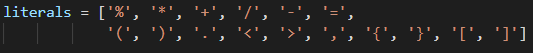
\includegraphics{literais.png}}
\caption{Declaração dos literais}
\label{fig}
\end{figure}  

\begin{figure}[htbp]
\centerline{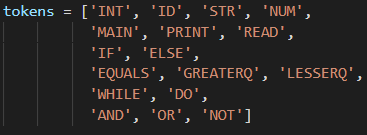
\includegraphics{tokens.png}}
\caption{Declaração dos tokens}
\label{fig}
\end{figure}  

\begin{figure}[htbp]
\centerline{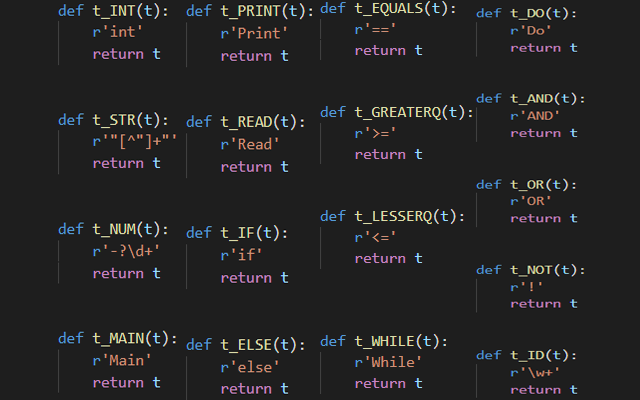
\includegraphics[scale=2.5]{funcoes_tokens.png}}
\caption{Declaração das funções dos tokens}
\label{fig}
\end{figure}  

\newpage
\begin{itemize}
     \item t\textunderscore INT - int;
     \item t\textunderscore STR - "string123", "ola", "@@@@@";
     \item t\textunderscore NUM - -5,2,0,77;
     \item t\textunderscore MAIN - Main;
     \item t\textunderscore PRINT - Print;
     \item t\textunderscore READ - Read;
     \item t\textunderscore IF - if;
     \item t\textunderscore ELSE - else;
     \item t\textunderscore EQUALS - ==;
     \item t\textunderscore GREATERQ - >=;
     \item t\textunderscore LESSERQ - <=;
     \item t\textunderscore WHILE - While;
     \item t\textunderscore DO - Do;
     \item t\textunderscore AND - AND;
     \item t\textunderscore OR - OR;
     \item t\textunderscore NOT - !;
     \item t\textunderscore ID - counter, x, var1.
  \end{itemize}

\newpage
Também é adicionado os tokens responsáveis por ignorar e detetar carateres inválidos, respetivamente:


\begin{figure}[htbp]
\centerline{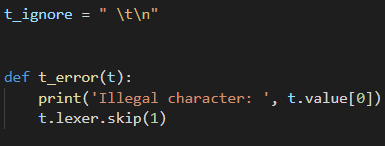
\includegraphics{ignore.png}}
\caption{ignore e error}
\label{fig}
\end{figure} 

\newpage
\subsection{Parser} \label{subsec:parser}
Esta parte do problema foi resolvido com 11 partes:

\begin{itemize}
     \item Principal;
     \item Declarations;
     \item Commands;
     \item Conditions;
     \item Expression;
     \item Term;
     \item Factors;
     \item ID/Error;
     \item Simple Arrays;
     \item Double Arrays;
     \item Parser Functions.
  \end{itemize}

\title{\textbf{Principal}}


\begin{figure}[htbp]
\centerline{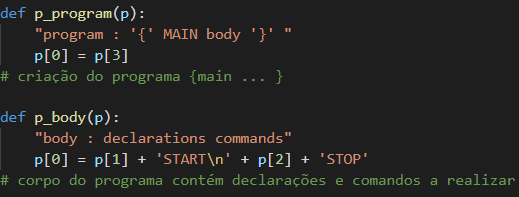
\includegraphics{principal.png}}
\caption{Principal}
\label{fig}
\end{figure} 

Existe 2 funções, 1 responsável pela descrição geral do programa, e a outra responsável pela declaração do corpo da função (respetivamente na imagem).

\newpage

\title{\textbf{Declarations}}


\begin{figure}[htbp]
\centerline{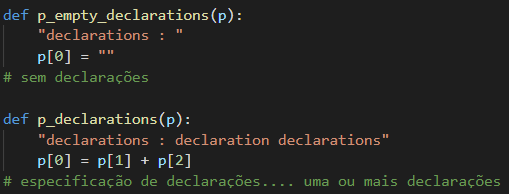
\includegraphics{declaracoes1.png}}
\caption{Excerto 1 das declarations}
\label{fig}
\end{figure} 
Nestas 2 funções é permitido ao utilizador fazer múltiplas declarações.\\

\begin{figure}[htbp]
\centerline{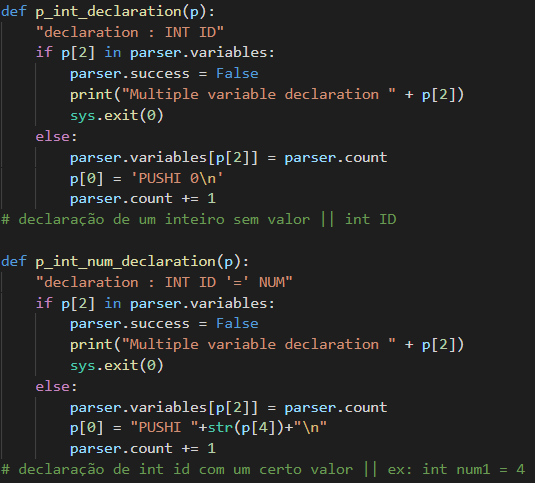
\includegraphics[scale=1]{declaracoes2.png}}
\caption{Excerto 2 das declarations}
\label{fig}
\end{figure} 

Nestas 2 funções é permitido ao utilizador declarar variáveis com ou sem inicialização.\\
Não é permitido existir múltiplas declarações da mesma variável.
\newpage

\title{\textbf{Commands}}
\begin{figure}[htbp]
\centerline{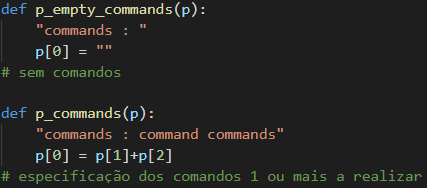
\includegraphics[scale=1]{commands1.png}}
\caption{Excerto 1 dos commands}
\label{fig}
\end{figure}

Nestas 2 funções é permitido declarar múltiplos comandos.\\
Os comandos que serão usados são os seguintes

\begin{itemize}
     \item Print;
     \item Read;
     \item If;
     \item Atribution;
     \item While-do.
  \end{itemize}

\newpage

\begin{figure}[htbp]
\centerline{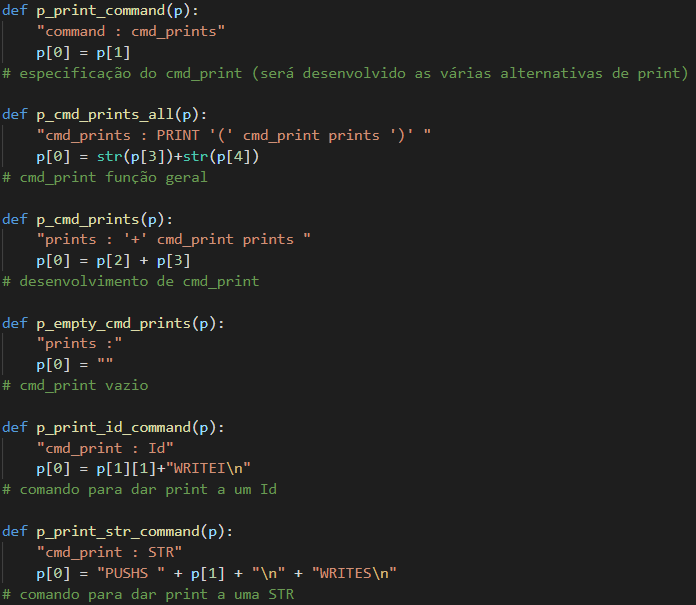
\includegraphics[scale=0.9]{commandsPrint.png}}
\caption{Excerto 2 dos commands (Print)}
\label{fig}
\end{figure}

Neste conjunto de funções é criada o comando "Print", que permite-nos dar print, ou a variáveis ou a strings.



\begin{figure}[htbp]
\centerline{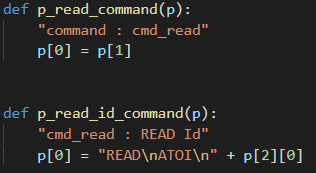
\includegraphics[scale=1]{commandsRead.png}}
\caption{Excerto 3 dos commands (Read)}
\label{fig}
\end{figure}

Neste conjunto de funções é criada o comando "Read", que permite-nos ler o input do utilizador.
\newpage

\begin{figure}[htbp]
\centerline{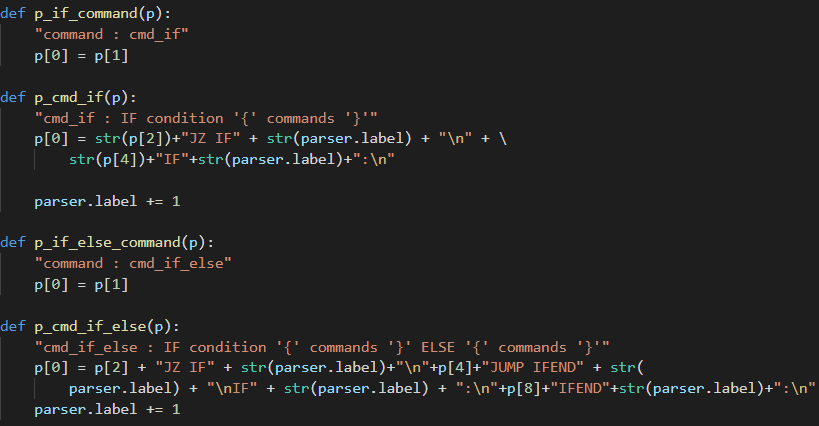
\includegraphics[scale=0.75]{commandsIf.png}}
\caption{Excerto 4 dos commands (If)}
\label{fig}
\end{figure}

Neste conjunto de funções é criada os comandos: "If" e "If Else".

\begin{figure}[htbp]
\centerline{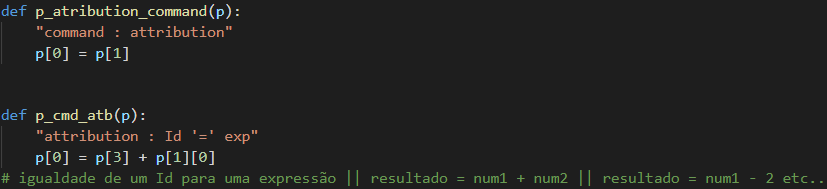
\includegraphics[scale=0.75]{commandsAtribuicao.png}}
\caption{Excerto 5 dos commands (Atribution)}
\label{fig}
\end{figure}

Neste conjunto de funções é criada o comando responsável por atribuir expressões às variáveis.

\begin{figure}[htbp]
\centerline{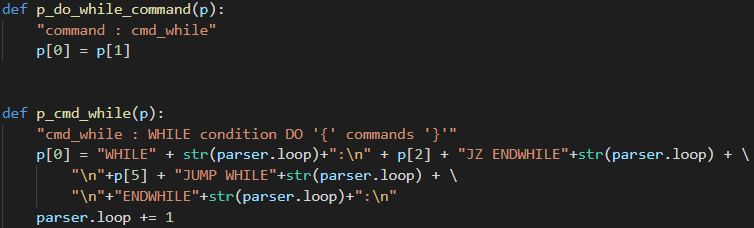
\includegraphics[scale=0.75]{commandsWhile.png}}
\caption{Excerto 6 dos commands (While-do)}
\label{fig}
\end{figure}

Neste conjunto de funções é criada o comando: While-do
\newpage


\title{\textbf{Conditions}}
\begin{figure}[htbp]
\centerline{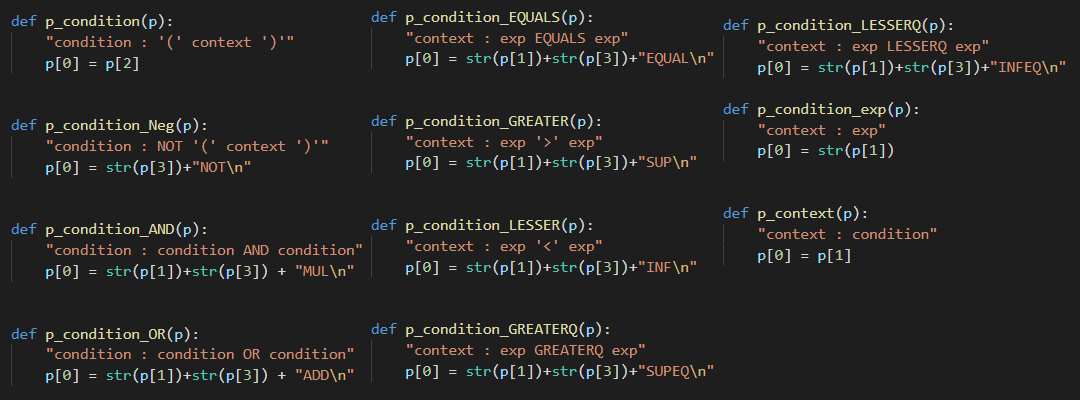
\includegraphics[scale=1.8]{conditions.png}}
\caption{Conditions}
\label{fig}
\end{figure}

Este conjunto de funções possuem as funções para gerar o essencial para as relações lógicas.
Existe:
\begin{itemize}
     \item Negação - 'Not';
     \item And - 'AND';
     \item Or - 'OR';
     \item Igualdade - 'EQUALS';
     \item Maior - ">'
     \item Menor - "<'
     \item Maior ou igual - 'GREATERQ';
     \item Menor ou igual - 'LESSERQ'.
  \end{itemize}

\title{\textbf{Expressions}}
\begin{figure}[htbp]
\centerline{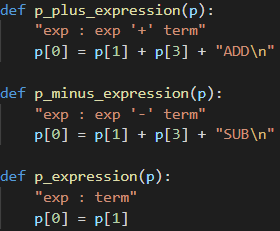
\includegraphics[scale=1]{expressoes.png}}
\caption{Expressions}
\label{fig}
\end{figure}

Estas funções permite a existência de aritmética simples.

\newpage
\title{\textbf{Terms}}
\begin{figure}[htbp]
\centerline{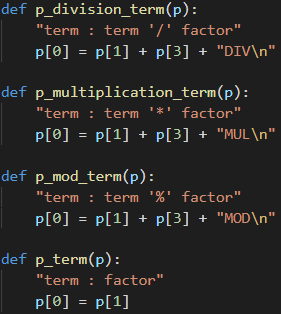
\includegraphics[scale=1]{termos.png}}
\caption{Terms}
\label{fig}
\end{figure}

Estas funções expandem a definição do "term" e permite a divisão, a multiplicação e o "MOD".\\

\title{\textbf{Factors}}
\begin{figure}[htbp]
\centerline{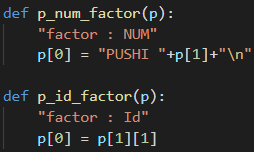
\includegraphics[scale=1]{factor.png}}
\caption{Factors}
\label{fig}
\end{figure}

Estas funções permite tornar, tanto um número, como um id, num fator que tem como objetivo ser usado nas contas

\newpage

\title{\textbf{ID/Error}}
\begin{figure}[htbp]
\centerline{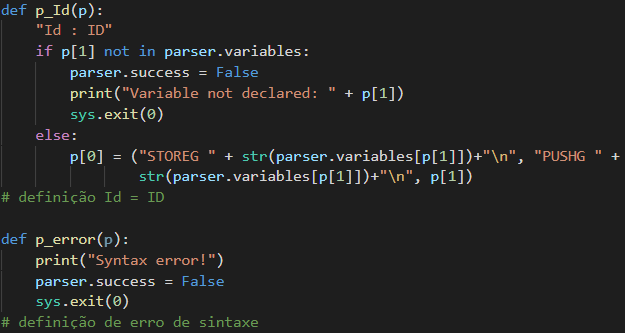
\includegraphics[scale=1]{idError.png}}
\caption{ID/Error}
\label{fig}
\end{figure}

A função id é responsável por 3 coisas, detetar se todas as variáveis foram declaradas (pois não faz sentido existir variáveis que não foram declaradas), dá store na stack e nas variáveis do sistema (que é as variáveis do parser).\\


\title{\textbf{Simple Arrays}}
\begin{figure}[htbp]
\centerline{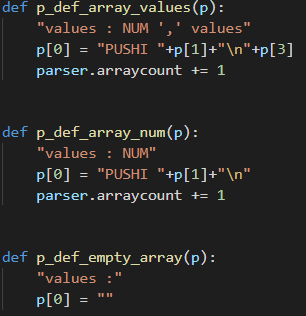
\includegraphics[scale=1]{simpleArrays1.png}}
\caption{Excerto 1 dos Arrays Simples}
\label{fig}
\end{figure}

Estas 3 funções são responsáveis por definir o termo "values" que é importante para os arrays. Pois é com este termo que podemos dar valores a cada index do array.

\newpage
\begin{figure}[htbp]
\centerline{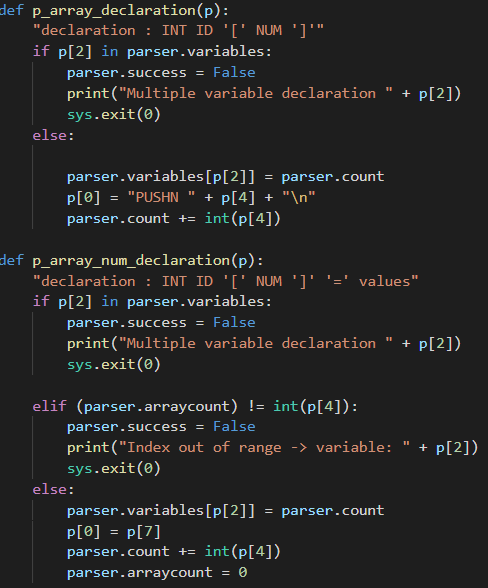
\includegraphics[scale=0.8]{simpleArrays2.png}}
\caption{Excerto 2 dos Arrays Simples}
\label{fig}
\end{figure}

Estas 2 funções são responsáveis por declarar os arrays, com ou sem inicialização. Caso que seja com inicialização, é necessário garantir que não que seja escrito for do array.\\

\begin{figure}[htbp]
\centerline{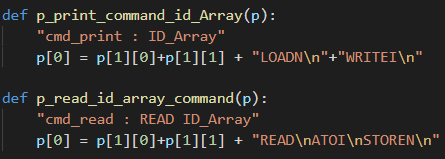
\includegraphics[scale=1]{simpleArrays3.png}}
\caption{Excerto 3 dos Arrays Simples}
\label{fig}
\end{figure}

Funções que permitem que a função "Read" e "Print" sejam utilizadas nos arrays simples também.\\

\newpage
\begin{figure}[htbp]
\centerline{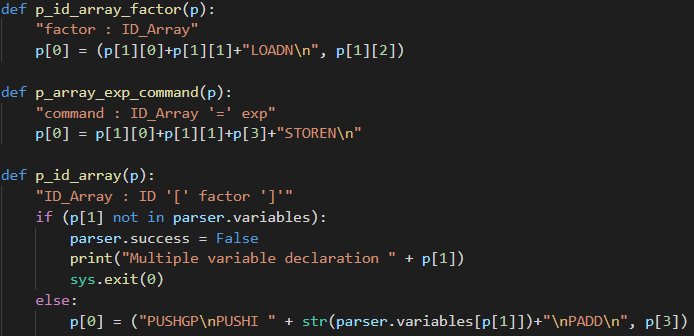
\includegraphics[scale=1]{simpleArrays4.png}}
\caption{Excerto 4 dos Arrays Simples}
\label{fig}
\end{figure}

A primeira função é responsável por permitir a utilização do array como um factor, a segunda é responsável por permitir que o array receba uma expressão. E for fim, é a função para atribuir o id ao array.


\title{\textbf{Double Arrays}}
\begin{figure}[htbp]
\centerline{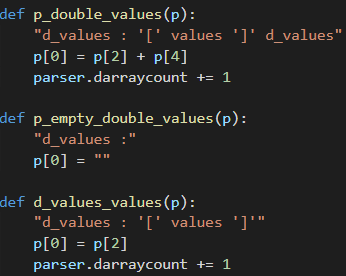
\includegraphics[scale=1]{doubleArrays1.png}}
\caption{Excerto 1 dos Arrays Duplos}
\label{fig}
\end{figure}

Estas 3 funções são responsáveis por definir o termo "d\textunderscore values" que é importante para os arrays duplos. Pois é com este termo que podemos dar valores a cada index de cada array.

\newpage

\begin{figure}[htbp]
\centerline{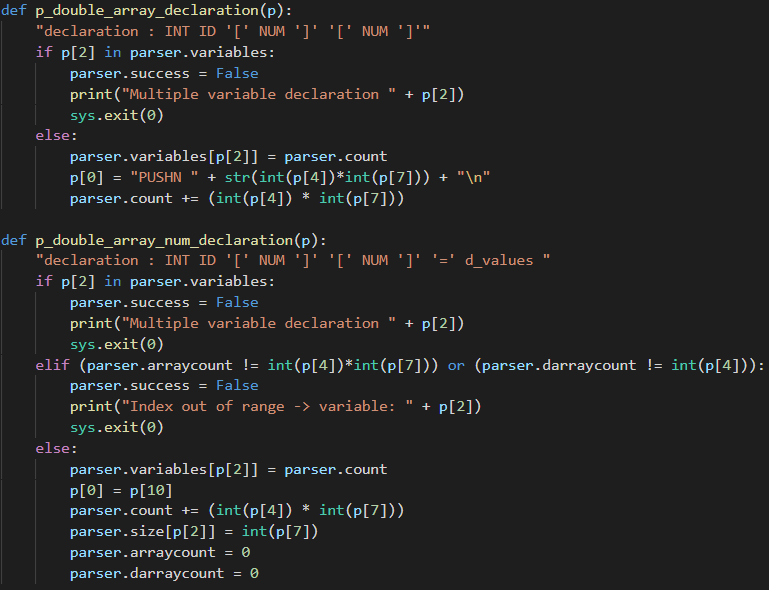
\includegraphics[scale=0.8]{doubleArrays2.png}}
\caption{Excerto 2 dos Arrays Duplos}
\label{fig}
\end{figure}

Estas 2 funções são responsáveis por declarar os arrays duplos, com ou sem inicialização. Caso que seja com inicialização, é necessário garantir que não que seja escrito for dos arrays.\\


\begin{figure}[htbp]
\centerline{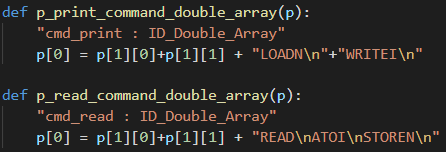
\includegraphics[scale=1]{doubleArrays3.png}}
\caption{Excerto 3 dos Arrays Duplos}
\label{fig}
\end{figure}

Funções que permitem que a função "Read" e "Print" sejam utilizadas nos arrays duplos também.\\

\newpage
\begin{figure}[htbp]
\centerline{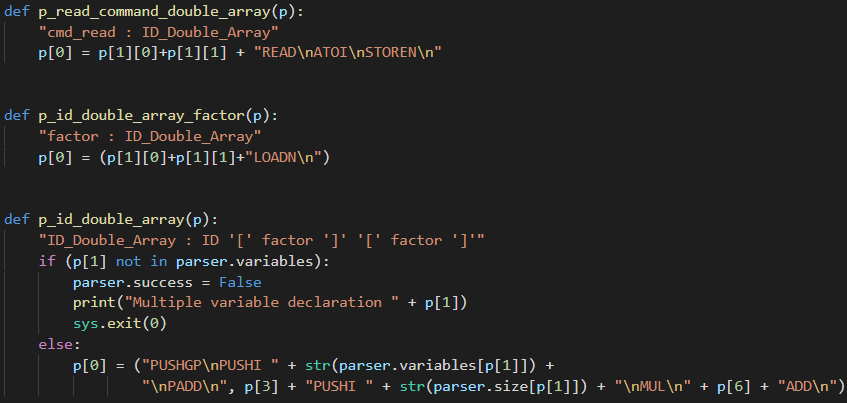
\includegraphics[scale=0.8]{doubleArrays4.png}}
\caption{Excerto 4 dos Arrays Duplos}
\label{fig}
\end{figure}

A primeira função é para permitir que o array duplo receba uma expressão, a segunda é responsável por permitir a utilização do array duplo como um factor. E for fim, é a função para atribuir o id ao array duplo.\\

\title{\textbf{Parser Functions}}
\begin{figure}[htbp]
\centerline{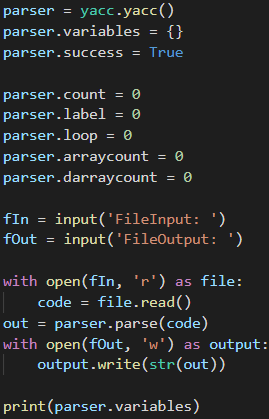
\includegraphics[scale=0.8]{parser.png}}
\caption{Parser}
\label{fig}
\end{figure}

Por fim, é utilizado o parser do yacc para compilar e criar o pseudo-código para executarmos na Máquina Virtual

\newpage
\section{Exemplos} \label{sec:ex}
\subsection{Exemplo 1} 

\begin{verbatim}
{
    Main 

    int num1 
    int num2 
    int num3
    int i = 0
    int resultado
    int array[4] 

    Print ("Armazenar valores de todas as operacoes basicas num array de dois num\n\n")
    Print ("Digite o primeiro num: \n ")
    Read num1
    Print ("Digite o segundo num: \n")
    Read num2 


    While !(num3 == 4) Do {

        if (num3 == 0){
            resultado = num1 + num2
            }
        if (num3 == 1){
            resultado = num1 - num2
            }
        if (num3 == 2){
            resultado = num1 * num2
            }
        if (num3 == 3){
            resultado = num1 / num2
            }
        array[num3] = resultado
        num3 = num3 +1
    }
    Print ("Valores do Array: \n")
    While !(i == 4) Do {
        Print(array[i])
        Print("\n")
        i = i +1
    }
}
\end{verbatim}

\newpage
\subsection{Exemplo 2}

\begin{verbatim}
{

    Main
    int valor
    int i = 0
    int j = 0
    int matriz[3][3] = [1,2,3][4,5,6][7,1,9]  
    int counter = 0

    Print ("Procurar um valor na matriz e contar quantas vezes ele aparece\n")
    Print("Digite o valor a procurar: \n")
    Read valor

    While (i < 3) Do {
        While ( j < 3) Do {
        if (valor == matriz[i][j]){

            valor = 1
            counter = counter + 1
            j = j + 1
        }
        else {
            j = j + 1
        }
        
        }
        i = i +1
        j = 0
    }

    if (valor == 1){

        Print("Valor encontrado: ")
        Print(valor)
        Print("\n numero de vezes encontrado: ")
        Print(counter)

    } else{
        
        Print("Valor nao encontrado\n")
    }

}
\end{verbatim}

\newpage

\section{Pseudo-Código Gerado} \label{sec:main1}
\subsection{Pseudo-Código - Exemplo 1}
\begin{verbatim}
PUSHI 0
PUSHI 0
PUSHI 0
PUSHI 0
PUSHI 0
PUSHN 4
START
PUSHS "Armazenar valores de todas as operacoes basicas num array de dois num\n\n"
WRITES
PUSHS "Digite o primeiro num: \n "
WRITES
READ
ATOI
STOREG 0
PUSHS "Digite o segundo num: \n"
WRITES
READ
ATOI
STOREG 1
WHILE0:
PUSHG 2
PUSHI 4
EQUAL
NOT
JZ ENDWHILE0
PUSHG 2
PUSHI 0
EQUAL
JZ IF0
PUSHG 0
PUSHG 1
ADD
STOREG 4
IF0:
PUSHG 2
PUSHI 1
EQUAL
JZ IF1
PUSHG 0
PUSHG 1
SUB
STOREG 4
IF1:
PUSHG 2
PUSHI 2
EQUAL
JZ IF2
PUSHG 0
PUSHG 1
MUL
STOREG 4
IF2:
PUSHG 2
PUSHI 3
EQUAL
JZ IF3
PUSHG 0
PUSHG 1
DIV
STOREG 4
IF3:
PUSHGP
PUSHI 5
PADD
PUSHG 2
PUSHG 4
STOREN
PUSHG 2
PUSHI 1
ADD
STOREG 2
JUMP WHILE0
ENDWHILE0:
PUSHS "Valores do Array: \n"
WRITES
WHILE1:
PUSHG 3
PUSHI 4
EQUAL
NOT
JZ ENDWHILE1
PUSHGP
PUSHI 5
PADD
PUSHG 3
LOADN
WRITEI
PUSHS "\n"
WRITES
PUSHG 3
PUSHI 1
ADD
STOREG 3
JUMP WHILE1
ENDWHILE1:
STOP
\end{verbatim}
\newpage
\subsection{Pseudo-Código - Exemplo 2}


\begin{verbatim}
PUSHI 0
PUSHI 0
PUSHI 0
PUSHI 1
PUSHI 2
PUSHI 3
PUSHI 4
PUSHI 5
PUSHI 6
PUSHI 7
PUSHI 1
PUSHI 9
PUSHI 0
START
PUSHS "Procurar um valor na matriz e contar quantas vezes ele aparece\n"
WRITES
PUSHS "Digite o valor a procurar: \n"
WRITES
READ
ATOI
STOREG 0
WHILE1:
PUSHG 1
PUSHI 3
INF
JZ ENDWHILE1
WHILE0:
PUSHG 2
PUSHI 3
INF
JZ ENDWHILE0
PUSHG 0
PUSHGP
PUSHI 3
PADD
PUSHG 1
PUSHI 3
MUL
PUSHG 2
ADD
LOADN
EQUAL
JZ IF0
PUSHI 1
STOREG 0
PUSHG 12
PUSHI 1
ADD
STOREG 12
PUSHG 2
PUSHI 1
ADD
STOREG 2
JUMP IFEND0
IF0:
PUSHG 2
PUSHI 1
ADD
STOREG 2
IFEND0:
JUMP WHILE0
ENDWHILE0:
PUSHG 1
PUSHI 1
ADD
STOREG 1
PUSHI 0
STOREG 2
JUMP WHILE1
ENDWHILE1:
PUSHG 0
PUSHI 1
EQUAL
JZ IF1
PUSHS "Valor encontrado: "
WRITES
PUSHG 0
WRITEI
PUSHS "\n numero de vezes encontrado: "
WRITES
PUSHG 12
WRITEI
JUMP IFEND1
IF1:
PUSHS "Valor nao encontrado\n"
WRITES
IFEND1:
STOP
\end{verbatim}


\newpage
\section{Código-Fonte} \label{sec:main1}
\subsection{tpLexer.py} \label{sec:lexer.py}
\begin{verbatim}
import ply.lex as lex

literals = ['%', '*', '+', '/', '-', '=',
            '(', ')', '.', '<', '>', ',', '{', '}', '[', ']']

tokens = ['INT', 'ID', 'STR', 'NUM',
          'MAIN', 'PRINT', 'READ',
          'IF', 'ELSE',
          'EQUALS', 'GREATERQ', 'LESSERQ',
          'WHILE', 'DO',
          'AND', 'OR', 'NOT']

def t_INT(t):
    r'int'
    return t

def t_STR(t):
    r'"[^"]+"'
    return t

def t_NUM(t):
    r'-?\d+'
    return t

def t_MAIN(t):
    r'Main'
    return t

def t_PRINT(t):
    r'Print'
    return t

def t_READ(t):
    r'Read'
    return t

def t_IF(t):
    r'if'
    return t

def t_ELSE(t):
    r'else'
    return t

def t_EQUALS(t):
    r'=='
    return t

def t_GREATERQ(t):
    r'>='
    return t

def t_LESSERQ(t):
    r'<='
    return t

def t_WHILE(t):
    r'While'
    return t

def t_DO(t):
    r'Do'
    return t

def t_AND(t):
    r'AND'
    return t

def t_OR(t):
    r'OR'
    return t

def t_NOT(t):
    r'!'
    return t

def t_ID(t):
    r'\w+'
    return t

t_ignore = " \t\n"

def t_error(t):
    print('Illegal character: ', t.value[0])
    t.lexer.skip(1)

lexer = lex.lex()


\end{verbatim}

\subsection{tpParser.py} \label{sec:parser.py}
\begin{verbatim}
import ply.yacc as yacc
import sys
from tp_lexer import tokens


def p_program(p):
    "program : '{' MAIN body '}' "
    p[0] = p[3]
# criação do programa {main ... }


def p_body(p):
    "body : declarations commands"
    p[0] = p[1] + 'START\n' + p[2] + 'STOP'
# corpo do programa contém declarações e comandos a realizar

# region DECLARATIONS FUNCTIONS


def p_empty_declarations(p):
    "declarations : "
    p[0] = ""
# sem declarações


def p_declarations(p):
    "declarations : declaration declarations"
    p[0] = p[1] + p[2]
# especificação de declarações.... uma ou mais declarações


def p_int_declaration(p):
    "declaration : INT ID"
    if p[2] in parser.variables:
        parser.success = False
        print("Multiple variable declaration " + p[2])
        sys.exit(0)
    else:
        parser.variables[p[2]] = parser.count
        p[0] = 'PUSHI 0\n'
        parser.count += 1
# declaração de um inteiro sem valor || int ID


def p_int_num_declaration(p):
    "declaration : INT ID '=' NUM"
    if p[2] in parser.variables:
        parser.success = False
        print("Multiple variable declaration " + p[2])
        sys.exit(0)
    else:
        parser.variables[p[2]] = parser.count
        p[0] = "PUSHI "+str(p[4])+"\n"
        parser.count += 1
# declaração de int id com um certo valor || ex: int num1 = 4

# endregion

# region ALL COMMANDS FUNCTIONS


def p_empty_commands(p):
    "commands : "
    p[0] = ""
# sem comandos


def p_commands(p):
    "commands : command commands"
    p[0] = p[1]+p[2]
# especificação dos comandos 1 ou mais a realizar

# region PRINT COMMAND FUNCTIONS


def p_print_command(p):
    "command : cmd_prints"
    p[0] = p[1]
# especificação do cmd_print (será desenvolvido as várias alternativas de print)


def p_cmd_prints_all(p):
    "cmd_prints : PRINT '(' cmd_print prints ')' "
    p[0] = str(p[3])+str(p[4])
# cmd_print função geral


def p_cmd_prints(p):
    "prints : '+' cmd_print prints "
    p[0] = p[2] + p[3]
# desenvolvimento de cmd_print


def p_empty_cmd_prints(p):
    "prints :"
    p[0] = ""
# cmd_print vazio


def p_print_id_command(p):
    "cmd_print : Id"
    p[0] = p[1][1]+"WRITEI\n"
# comando para dar print a um Id


def p_print_str_command(p):
    "cmd_print : STR"
    p[0] = "PUSHS " + p[1] + "\n" + "WRITES\n"
# comando para dar print a uma STR

# endregion

# region READ COMMAND FUNCTIONS


def p_read_command(p):
    "command : cmd_read"
    p[0] = p[1]


def p_read_id_command(p):
    "cmd_read : READ Id"
    p[0] = "READ\nATOI\n" + p[2][0]


# endregion

# region IF COMMAND // IF ELSE COMMAND FUNCTIONS


def p_if_command(p):
    "command : cmd_if"
    p[0] = p[1]


def p_cmd_if(p):
    "cmd_if : IF condition '{' commands '}'"
    p[0] = str(p[2])+"JZ IF" + str(parser.label) + "\n" + \
        str(p[4])+"IF"+str(parser.label)+":\n"

    parser.label += 1


def p_if_else_command(p):
    "command : cmd_if_else"
    p[0] = p[1]


def p_cmd_if_else(p):
    "cmd_if_else : IF condition '{' commands '}' ELSE '{' commands '}'"
    p[0] = p[2] + "JZ IF" + str(parser.label)+"\n"+p[4]+"JUMP IFEND" + str(
        parser.label) + "\nIF" + str(parser.label) + ":\n"+p[8]+"IFEND"+str(parser.label)+":\n"
    parser.label += 1


# endregion

def p_atribution_command(p):
    "command : attribution"
    p[0] = p[1]


def p_cmd_atb(p):
    "attribution : Id '=' exp"
    p[0] = p[3] + p[1][0]
# igualdade de um Id para uma expressão || resultado = num1 + num2 || resultado = num1 - 2 etc..

# region WHILE DO FUNCTIONS


def p_do_while_command(p):
    "command : cmd_while"
    p[0] = p[1]


def p_cmd_while(p):
    "cmd_while : WHILE condition DO '{' commands '}'"
    p[0] = "WHILE" + str(parser.loop)+":\n" + p[2] + "JZ ENDWHILE"+str(parser.loop) + \
        "\n"+p[5] + "JUMP WHILE"+str(parser.loop) + \
        "\n"+"ENDWHILE"+str(parser.loop)+":\n"
    parser.loop += 1

# endregion

# endregion


# region CONDITIONS FUNCTIONS

def p_condition(p):
    "condition : '(' context ')'"
    p[0] = p[2]


def p_condition_Neg(p):
    "condition : NOT '(' context ')'"
    p[0] = str(p[3])+"NOT\n"


def p_condition_AND(p):
    "condition : condition AND condition"
    p[0] = str(p[1])+str(p[3]) + "MUL\n"


def p_condition_OR(p):
    "condition : condition OR condition"
    p[0] = str(p[1])+str(p[3]) + "ADD\n"


def p_condition_EQUALS(p):
    "context : exp EQUALS exp"
    p[0] = str(p[1])+str(p[3])+"EQUAL\n"


def p_condition_GREATER(p):
    "context : exp '>' exp"
    p[0] = str(p[1])+str(p[3])+"SUP\n"


def p_condition_LESSER(p):
    "context : exp '<' exp"
    p[0] = str(p[1])+str(p[3])+"INF\n"


def p_condition_GREATERQ(p):
    "context : exp GREATERQ exp"
    p[0] = str(p[1])+str(p[3])+"SUPEQ\n"


def p_condition_LESSERQ(p):
    "context : exp LESSERQ exp"
    p[0] = str(p[1])+str(p[3])+"INFEQ\n"


def p_context(p):
    "context : condition"
    p[0] = p[1]

# endregion

# region EXPRESSION FUNCTIONS


def p_plus_expression(p):
    "exp : exp '+' term"
    p[0] = p[1] + p[3] + "ADD\n"


def p_minus_expression(p):
    "exp : exp '-' term"
    p[0] = p[1] + p[3] + "SUB\n"


def p_expression(p):
    "exp : term"
    p[0] = p[1]

# endregion

# region TERM FUNCTIONS


def p_division_term(p):
    "term : term '/' factor"
    p[0] = p[1] + p[3] + "DIV\n"


def p_multiplication_term(p):
    "term : term '*' factor"
    p[0] = p[1] + p[3] + "MUL\n"


def p_mod_term(p):
    "term : term '%' factor"
    p[0] = p[1] + p[3] + "MOD\n"


def p_term(p):
    "term : factor"
    p[0] = p[1]
# endregion

# region FACTORS FUNCTIONS


def p_num_factor(p):
    "factor : NUM"
    p[0] = "PUSHI "+p[1]+"\n"


def p_id_factor(p):
    "factor : Id"
    p[0] = p[1][1]

# endregion


def p_Id(p):
    "Id : ID"
    if p[1] not in parser.variables:
        parser.success = False
        print("Variable not declared: " + p[1])
        sys.exit(0)
    else:
        p[0] = ("STOREG " + str(parser.variables[p[1]])+"\n", "PUSHG " +
                str(parser.variables[p[1]])+"\n", p[1])
# definição Id = ID


def p_error(p):
    print("Syntax error!")
    parser.success = False
    sys.exit(0)
# definição de erro de sintaxe

# region ALL FUNCTIONS RELATED TO SIMPLE ARRAYS


def p_def_array_values(p):
    "values : NUM ',' values"
    p[0] = "PUSHI "+p[1]+"\n"+p[3]
    parser.arraycount += 1


def p_def_array_num(p):
    "values : NUM"
    p[0] = "PUSHI "+p[1]+"\n"
    parser.arraycount += 1


def p_def_empty_array(p):
    "values :"
    p[0] = ""


def p_array_declaration(p):
    "declaration : INT ID '[' NUM ']'"
    if p[2] in parser.variables:
        parser.success = False
        print("Multiple variable declaration " + p[2])
        sys.exit(0)
    else:

        parser.variables[p[2]] = parser.count
        p[0] = "PUSHN " + p[4] + "\n"
        parser.count += int(p[4])


def p_array_num_declaration(p):
    "declaration : INT ID '[' NUM ']' '=' values"
    if p[2] in parser.variables:
        parser.success = False
        print("Multiple variable declaration " + p[2])
        sys.exit(0)

    elif (parser.arraycount) != int(p[4]):
        parser.success = False
        print("Index out of range -> variable: " + p[2])
        sys.exit(0)
    else:
        parser.variables[p[2]] = parser.count
        p[0] = p[7]
        parser.count += int(p[4])
        parser.arraycount = 0


def p_print_command_id_Array(p):
    "cmd_print : ID_Array"
    p[0] = p[1][0]+p[1][1] + "LOADN\n"+"WRITEI\n"


def p_read_id_array_command(p):
    "cmd_read : READ ID_Array"
    p[0] = p[1][0]+p[1][1] + "READ\nATOI\nSTOREN\n"


def p_id_array_factor(p):
    "factor : ID_Array"
    p[0] = (p[1][0]+p[1][1]+"LOADN\n", p[1][2])


def p_condition_exp(p):
    "context : exp"
    p[0] = str(p[1])


def p_array_exp_command(p):
    "command : ID_Array '=' exp"
    p[0] = p[1][0]+p[1][1]+p[3]+"STOREN\n"


def p_id_array(p):
    "ID_Array : ID '[' factor ']'"
    if (p[1] not in parser.variables):
        parser.success = False
        print("Multiple variable declaration " + p[1])
        sys.exit(0)
    else:
        p[0] = ("PUSHGP\nPUSHI " + str(parser.variables[p[1]])+"\nPADD\n", p[3])

        # endregion


# region ALL FUNCTIONS RELATED TO DOUBLE ARRAYS

def p_double_values(p):
    "d_values : '[' values ']' d_values"
    p[0] = p[2] + p[4]
    parser.darraycount += 1


def p_empty_double_values(p):
    "d_values :"
    p[0] = ""


def d_values_values(p):
    "d_values : '[' values ']'"
    p[0] = p[2]
    parser.darraycount += 1


def p_double_array_declaration(p):
    "declaration : INT ID '[' NUM ']' '[' NUM ']'"
    if p[2] in parser.variables:
        parser.success = False
        print("Multiple variable declaration " + p[2])
        sys.exit(0)
    else:
        parser.variables[p[2]] = parser.count
        p[0] = "PUSHN " + str(int(p[4])*int(p[7])) + "\n"
        parser.count += (int(p[4]) * int(p[7]))

def p_double_array_num_declaration(p):
    "declaration : INT ID '[' NUM ']' '[' NUM ']' '=' d_values "
    if p[2] in parser.variables:
        parser.success = False
        print("Multiple variable declaration " + p[2])
        sys.exit(0)
    elif (parser.arraycount != int(p[4])*int(p[7])) or (parser.darraycount != int(p[4])):
        parser.success = False
        print("Index out of range -> variable: " + p[2])
        sys.exit(0)
    else:
        parser.variables[p[2]] = parser.count
        p[0] = p[10]
        parser.count += (int(p[4]) * int(p[7]))
        parser.size[p[2]] = int(p[7])
        parser.arraycount = 0
        parser.darraycount = 0


def p_double_array_exp_command(p):
    "command : ID_Double_Array '=' exp"
    p[0] = p[1][0]+p[1][1]+p[3]+"STOREN\n"


def p_print_command_double_array(p):
    "cmd_print : ID_Double_Array"
    p[0] = p[1][0]+p[1][1] + "LOADN\n"+"WRITEI\n"


def p_read_command_double_array(p):
    "cmd_read : ID_Double_Array"
    p[0] = p[1][0]+p[1][1] + "READ\nATOI\nSTOREN\n"


def p_id_double_array_factor(p):
    "factor : ID_Double_Array"
    p[0] = (p[1][0]+p[1][1]+"LOADN\n")


def p_id_double_array(p):
    "ID_Double_Array : ID '[' factor ']' '[' factor ']'"
    if (p[1] not in parser.variables):
        parser.success = False
        print("Multiple variable declaration " + p[1])
        sys.exit(0)
    else:
        p[0] = ("PUSHGP\nPUSHI " + str(parser.variables[p[1]]) +
                "\nPADD\n", p[3] + "PUSHI " + str(parser.size[p[1]]) + "\nMUL\n" + p[6] + "ADD\n")


# endregion

parser = yacc.yacc()
parser.variables = {}
parser.success = True

parser.count = 0
parser.label = 0
parser.loop = 0
parser.size = {}
parser.arraycount = 0
parser.darraycount = 0

fIn = input('FileInput: ')
fOut = input('FileOutput: ')

with open(fIn, 'r') as file:
    code = file.read()
out = parser.parse(code)
with open(fOut, 'w') as output:
    output.write(str(out))

print(parser.variables)

\end{verbatim}

\end{document} 
